% ---
% school: "college"
% level: "8eme"
% section: null
% chapter: "التناظر المركزي"
% source: "Axiomaths"
% title: "تركيب : دائرة ومستطيل"
% country: "Tunisie"
% year: 2026
% professor: "Axiomaths"
% difficulty: "Moyen"
% points: null
% tags: ["symetrie-centrale", "symetrie-axiale", "cercle", "rectangle", "angles", "synthese"]
% ---
% Exercice 11/19 de la série 8ème « التناظر المركزي » (statement + \axsol + solution). Compiler avec XeLaTeX + axiomath.sty (+ axiomaths-logo.png).
\documentclass[12pt,a4paper]{article}
\usepackage[level=8b,color=15803D]{axiomath}
\usetikzlibrary{arrows.meta}
\newcommand{\cm}{\,\mathrm{cm}}
\axsetup{title={التناظر المركزي}, corrige}

\begin{document}

\begin{corr}[title={تركيب : دائرة ومستطيل}, stars=3, source={Axiomaths}]
$\mathcal{C}$ دائرة مركزها $O$ وشعاعها $3\cm$ و $[AB]$ قطر لها. $M$ نقطة من $\mathcal{C}$ حيث $\widehat{AOM}=40^\circ$ ، $N$ مناظرة $M$ بالنسبة إلى $(AB)$ ، و $M'$ و $N'$ مناظرتا $M$ و $N$ بالنسبة إلى $O$.
\begin{enumerate}
  \item ابنِ الشكل. بين أن $N$ و $M'$ و $N'$ تنتمي إلى $\mathcal{C}$.
  \item احسب $\widehat{MON}$.
  \item بين أن $MNM'N'$ مستطيل.
  \item احسب $\widehat{OMN}$ و $\widehat{OMN'}$ ، ثم تحقق أن $\widehat{NMN'}=90^\circ$.
  \item بين أن $(AB)$ محور تناظر للمستطيل $MNM'N'$.
\end{enumerate}
\axsol
\begin{enumerate}[itemsep=14pt]
  \item\leavevmode
  \begin{prop}[التناظر يحفظ الأطوال]
  $O$ تنتمي إلى $(AB)$ ، فمناظرتها بالنسبة إلى $(AB)$ هي $O$ نفسها. إذن \ib{$ON=OM=3\cm$}.
  \end{prop}
  والتناظر المركزي يحفظ الأطوال أيضا ومركزه $O$ : $OM'=OM=3\cm$ و $ON'=ON=3\cm$. النقاط $N$ و $M'$ و $N'$ تبعد $3\cm$ عن $O$ : إنها تنتمي إلى $\mathcal{C}$.
  \begin{center}
  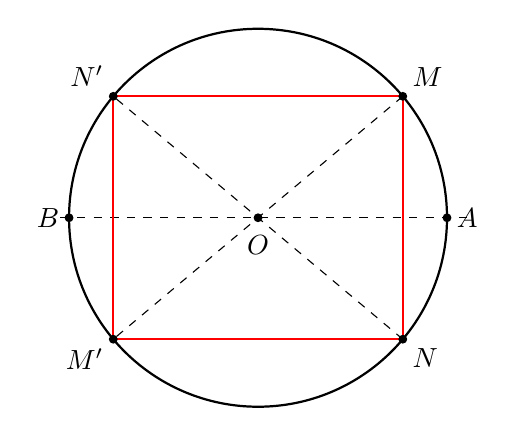
\begin{tikzpicture}[scale=0.8]
    \draw[thick] (0,0) circle (3);
    \draw[dashed] (-3.4,0)--(3.4,0);
    \draw[thick,red] (2.298,1.928)--(2.298,-1.928)--(-2.298,-1.928)--(-2.298,1.928)--cycle;
    \draw[dashed] (2.298,1.928)--(-2.298,-1.928);
    \draw[dashed] (2.298,-1.928)--(-2.298,1.928);
    \fill (0,0) circle (2pt) node[below=3pt] {$O$};
    \fill (3,0) circle (2pt) node[right] {$A$};
    \fill (-3,0) circle (2pt) node[left] {$B$};
    \fill (2.298,1.928) circle (2pt) node[above right] {$M$};
    \fill (2.298,-1.928) circle (2pt) node[below right] {$N$};
    \fill (-2.298,-1.928) circle (2pt) node[below left] {$M'$};
    \fill (-2.298,1.928) circle (2pt) node[above left] {$N'$};
  \end{tikzpicture}
  \end{center}
  \item التناظر المحوري يحفظ قيس الزوايا، فـ $\widehat{AON}=\widehat{AOM}=40^\circ$. و $M$ و $N$ على جهتين مختلفتين من $(AB)$ ، إذن :
  \[\widehat{MON}=40^\circ+40^\circ=80^\circ\]
  \item \begin{prop}[قطرا متوازي الأضلاع]
  رباعي قطراه لهما نفس المنتصف هو متوازي أضلاع ؛ وإذا كان قطراه متقايسين فهو \ib{مستطيل}.
  \end{prop}
  قطرا $MNM'N'$ هما $[MM']$ و $[NN']$. $O$ منتصف $[MM']$ لأن $M'=S_O(M)$ ، و $O$ منتصف $[NN']$ لأن $N'=S_O(N)$ : نفس المنتصف.
  و $MM'=2\times3=6\cm=NN'$ (قطران للدائرة) : القطران متقايسان. إذن $MNM'N'$ مستطيل.
  \item المثلث $OMN$ متقايس الضلعين رأسه $O$ وزاويته في الرأس $80^\circ$ :
  \[\widehat{OMN}=\dfrac{180^\circ-80^\circ}{2}=50^\circ\]
  $N$ و $O$ و $N'$ على استقامة واحدة، إذن $\widehat{MON'}=180^\circ-80^\circ=100^\circ$. المثلث $OMN'$ متقايس الضلعين رأسه $O$ :
  \[\widehat{OMN'}=\dfrac{180^\circ-100^\circ}{2}=40^\circ\]
  و $O$ داخل الزاوية $\widehat{NMN'}$ ، إذن $\widehat{NMN'}=50^\circ+40^\circ=90^\circ$ : زاوية قائمة كما في كل مستطيل.
  \item $N=S_{(AB)}(M)$ ، فـ $(AB)$ هو محور القطعة $[MN]$.
  التناظر المركزي $S_O$ يحوّل $(AB)$ إلى نفسه (مستقيم يمر من $O$) ، و $M$ إلى $M'$ و $N$ إلى $N'$ ؛ فيحوّل محور $[MN]$ إلى محور $[M'N']$. إذن $(AB)$ هو أيضا محور $[M'N']$.
  وهكذا $S_{(AB)}$ يبدّل $M$ و $N$ ، ويبدّل $M'$ و $N'$ : \ib{المستطيل ينطبق على نفسه}، فـ $(AB)$ محور تناظره.
\end{enumerate}
\textbf{الفكرة :} للمستطيل مركز تناظر ومحوران : $O$ ، و $(AB)$ ، والمستقيم العمودي عليه في $O$. \quad \textbf{انتبه :} قارن مع تمرين المراكز والمحاور (متوازي الأضلاع العادي لا محور له).
\end{corr}

\end{document}
